\NoBgThispage
\section{Struttura Generale dell'Applicazione}
Il codice sorgente nel package \texttt{src/main/java} è suddiviso in tre Macro-package:
\begin{itemize}
    \item \texttt{client} nel quale sono presenti il package \texttt{GUI} che contiene le classi
          dell'interfaccia grafica, \texttt{mainPackage} che contiene la classe punto di ingresso dell'applicazione e \texttt{models} che contiene le classi responsabili
          della connessione remota ai servizi RMI presenti nel modulo Server;
    \item \texttt{server} contiene le classi che implementano i servizi RMI, la classe che si occupa della connessione al database e la principale che fa
          partire il server;
    \item \texttt{shared} contiene le classi che sono condivise tra il modulo Client e il modulo Server, come ad esempio le interfacce dei servizi RMI,
          i record dei dati e le classi che implementano funzioni di utilità.
\end{itemize}

\begin{figure}[H]
    \centering
    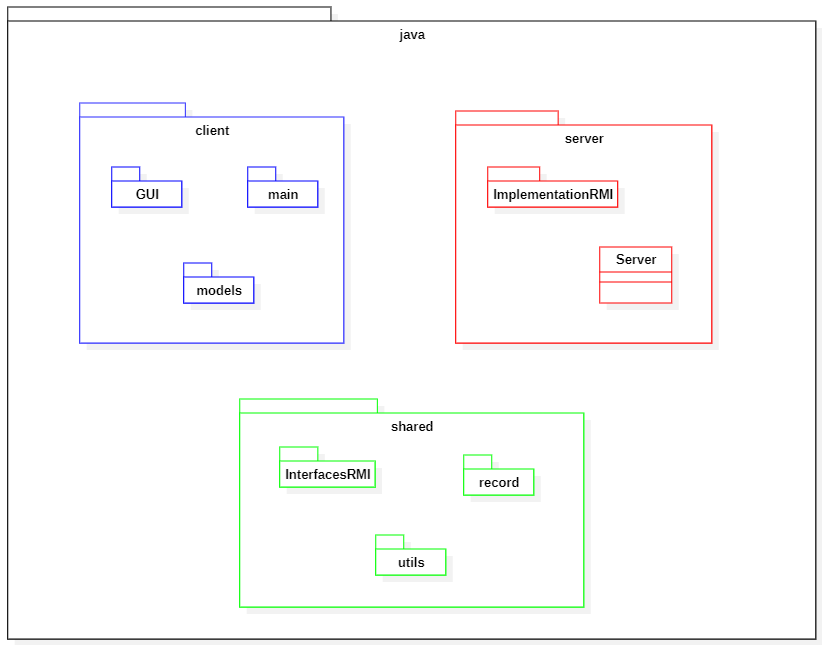
\includegraphics[width=0.8\textwidth]{img/packageStructure.png}
    \caption{Struttura dei package dell'applicazione.}
\end{figure}